%% This is file `sample-sigconf.tex',
%% generated with the docstrip utility.
%%
%% The original source files were:
%%
%% samples.dtx  (with options: `sigconf')
%% 
%% IMPORTANT NOTICE:
%% 
%% For the copyright see the source file.
%% 
%% Any modified versions of this file must be renamed
%% with new filenames distinct from sample-sigconf.tex.
%% 
%% For distribution of the original source see the terms
%% for copying and modification in the file samples.dtx.
%% 
%% This generated file may be distributed as long as the
%% original source files, as listed above, are part of the
%% same distribution. (The sources need not necessarily be
%% in the same archive or directory.)
%%
%% Commands for TeXCount
%TC:macro \cite [option:text,text]
%TC:macro \citep [option:text,text]
%TC:macro \citet [option:text,text]
%TC:envir table 0 1
%TC:envir table* 0 1
%TC:envir tabular [ignore] word
%TC:envir displaymath 0 word
%TC:envir math 0 word
%TC:envir comment 0 0
%%
%%
%% The first command in your LaTeX source must be the \documentclass command.
\documentclass[sigconf]{acmart}
%% NOTE that a single column version is required for 
%% submission and peer review. This can be done by changing
%% the \doucmentclass[...]{acmart} in this template to 
%% \documentclass[manuscript,screen]{acmart}
%% 
%% To ensure 100% compatibility, please check the white list of
%% approved LaTeX packages to be used with the Master Article Template at
%% https://www.acm.org/publications/taps/whitelist-of-latex-packages 
%% before creating your document. The white list page provides 
%% information on how to submit additional LaTeX packages for 
%% review and adoption.
%% Fonts used in the template cannot be substituted; margin 
%% adjustments are not allowed.

\usepackage{subcaption}
\usepackage{tikz}
\usetikzlibrary {arrows.meta, automata, positioning, fit}
\usepackage{url}
\usepackage{algorithm}
\usepackage{algpseudocode}

%%
%% \BibTeX command to typeset BibTeX logo in the docs
\AtBeginDocument{%
  \providecommand\BibTeX{{%
    \normalfont B\kern-0.5em{\scshape i\kern-0.25em b}\kern-0.8em\TeX}}}

%% Rights management information.  This information is sent to you
%% when you complete the rights form.  These commands have SAMPLE
%% values in them; it is your responsibility as an author to replace
%% the commands and values with those provided to you when you
%% complete the rights form.
\setcopyright{acmcopyright}
\copyrightyear{2022}
\acmYear{2022}
\acmDOI{XXXXXXX.XXXXXXX}

%% These commands are for a PROCEEDINGS abstract or paper.
\acmConference[Conference acronym 'XX]{Make sure to enter the correct
  conference title from your rights confirmation emai}{June 03--05,
  2018}{Woodstock, NY}
%
%  Uncomment \acmBooktitle if th title of the proceedings is different
%  from ``Proceedings of ...''!
%
%\acmBooktitle{Woodstock '18: ACM Symposium on Neural Gaze Detection,
%  June 03--05, 2018, Woodstock, NY} 
\acmPrice{15.00}
\acmISBN{978-1-4503-XXXX-X/22/12}
% set algorithmicx

\renewcommand{\algorithmicrequire}{\textbf{Input:}}  % Use Input in the format of Algorithm  
\renewcommand{\algorithmicensure}{\textbf{Output:}} % Use Output in the format of Algorithm 


\newcommand*{\red}[1]{\textcolor{red}{#1}}

\newcommand*{\myvec}[1]{\bar{#1}}
\newcommand*{\regex}{\mathcal{R}}
\newcommand*{\strsort}{\verb|Str|}
\newcommand*{\intsort}{\verb|Int|}
\newcommand*{\lan}{\mathcal{L}}
\newcommand*{\highlight}[1]{\textbf{\textit{#1}}}
\newcommand*{\aut}{\mathcal{A}}
\newcommand*{\algfun}[1]{\texttt{#1}}
\newcommand*{\strlen}[1]{\texttt{len}(#1)}

%%
%% Submission ID.
%% Use this when submitting an article to a sponsored event. You'll
%% receive a unique submission ID from the organizers
%% of the event, and this ID should be used as the parameter to this command.
%%\acmSubmissionID{123-A56-BU3}

%%
%% For managing citations, it is recommended to use bibliography
%% files in BibTeX format.
%%
%% You can then either use BibTeX with the ACM-Reference-Format style,
%% or BibLaTeX with the acmnumeric or acmauthoryear sytles, that include
%% support for advanced citation of software artefact from the
%% biblatex-software package, also separately available on CTAN.
%%
%% Look at the sample-*-biblatex.tex files for templates showcasing
%% the biblatex styles.
%%

%%
%% The majority of ACM publications use numbered citations and
%% references.  The command \citestyle{authoryear} switches to the
%% "author year" style.
%%
%% If you are preparing content for an event
%% sponsored by ACM SIGGRAPH, you must use the "author year" style of
%% citations and references.
%% Uncommenting
%% the next command will enable that style.
%%\citestyle{acmauthoryear}

%%
%% end of the preamble, start of the body of the document source.
\begin{document}

%%
%% The "title" command has an optional parameter,
%% allowing the author to define a "short title" to be used in page headers.
\title{Efficient Methods for Solving String Constraints with Large Repetition Bound}

%%
%% The "author" command and its associated commands are used to define
%% the authors and their affiliations.
%% Of note is the shared affiliation of the first two authors, and the
%% "authornote" and "authornotemark" commands
%% used to denote shared contribution to the research.
\author{DengHang Hu}
% \authornote{Both authors contributed equally to this research.}
\affiliation{%
  \institution{State Key Laboratory of Computer Science,
    Institute of Software, Chinese Academy of Sciences}
  \city{}
  \country{}
}
\email{hudh@ios.ac.cn}

\author{Zhilin Wu}
% \authornote{Both authors contributed equally to this research.}
\affiliation{%
  \institution{State Key Laboratory of Computer Science,
    Institute of Software, Chinese Academy of Sciences}
  \city{}
  \country{}
}
\email{wuzl@ios.ac.cn}



%%
%% The abstract is a short summary of the work to be presented in the
%% article.
\begin{abstract}
  Regular expression with large repetition bounds frequently appears in the real world. However, state-of-art string solvers can not efficiently solve string constraints with large
  repetition bounds, which slows down string constraint
  applications like formal verification and symbolic execution. In this paper, we
  propose a new systematic algorithm based on the decision procedure in our previous work to solve the problem efficiently. We use
  heuristic ways like over-approximation and under-approximation to accelerate the search. Further, we extract amounts of regex expressions with repetition
  times from real-world programs and generate a significant benchmark. We evaluate the algorithm's performance on our generated
  and developed benchmarks. The result shows that our solver outperforms the state-of-art string solvers.

\end{abstract}

%%
%% The code below is generated by the tool at http://dl.acm.org/ccs.cfm.
%% Please copy and paste the code instead of the example below.
%%
% \begin{CCSXML}
% <ccs2012>
%    <concept>
%        <concept_id>10003752.10003766.10003776</concept_id>
%        <concept_desc>Theory of computation~Regular languages</concept_desc>
%        <ignificance>500</concept_significance>
%        </concept>
%  </ccs2012>
% \end{CCSXML}

\ccsdesc[500]{Theory of computation~Regular languages}

%%
%% Keywords. The author(s) should pick words that accurately describe
%% the work being presented. Separate the keywords with commas.
\keywords{string constraints, cost-enriched automata, regex expression, bounded repetition}

%% A "teaser" image appears between the author and affiliation
%% information and the body of the document, and typically spans the
%% page.
% \begin{teaserfigure}
%   \includegraphics[width=\textwidth]{sampleteaser}
%   \caption{Seattle Mariners at Spring Training, 2010.}
%   \Description{Enjoying the baseball game from the third-base
%   seats. Ichiro Suzuki preparing to bat.}
%   \label{fig:teaser}
% \end{teaserfigure}

% \received{20 February 2007}
% \received[revised]{12 March 2009}
% \received[accepted]{5 June 2009}

%%
%% This command processes the author and affiliation and title
%% information and builds the first part of the formatted document.
\maketitle

\section{Introduction}
Regular expressions are widely used in programming languages such as Javascript and Python. About 30–40 \% of Java, JavaScript, and Python software uses regex
matching\cite{redos_fse2019}. To find
potential software bugs automatically, many researchers prefer to use one of the
formal verification technology - symbolic execution \cite{symbolic_pldi2021}. Symbolic execution views symbolic paths as multi-theories
constraints and uses a constraints solver to solve these constraints. Thus the
efficiency and the ability of the constraints solver are vitally important.
However, the string theory is one of the most challenging theories in multi-theory constraints because it is easy to be undecidable\cite{undecidable_2016}. So the string constraints solver with the higher
ability (support more operators) usually performs slower. Most solvers try very hard to improve efficiency. For example, Z3 and cvc5 append many heuristic
derivation rules to speed up their search in the DPLL framework. Trau+ proposes
a new model called flat automaton and uses the CEGAR framework to under-approximate
and over-approximate the string constraints again and again.
Unfortunately, the string solvers above perform poorly when the string constraints contain large repetition bound. The DPLL-framework string solvers prefer to
search model strings with smaller lengths, but large repetition bound most often stands
for considerable model string lengths. The automaton-based solvers
unwind the automaton naively, so the search space of the unwound automaton is
exponential of the repetition bound. To address this issue, we extend
cost-enriched finite automaton\cite{atva2020} whose search space is linear to the
repetition bound. Our main contributions are:
\begin{enumerate}
  \item We extend cost-enriched finite automaton to model the extended regular expression with large repetition bound.
  \item We devise an efficient algorithm to solve string constraints with large repetition bound with the new automaton model.
  \item We generate many instances with large repetition bound from real-word regular expressions.
  \item We implemented our efficient algorithm on ostrich and compared it with state-of-art string solvers. The result shows the superiority of our automaton model and algorithm.
\end{enumerate}
%TODO: list the main contributions
The structure of this paper is as follows: We introduce some abbreviations and concepts in section \ref{sec:pre} and introduce the syntax and semantics of the string theory logic in section \ref{sec:str_t}. Then we develop cost-enriched finite automaton model and its operations at section \ref{sec:cefa}. The efficient algorithm is discussed in section \ref{sec:solve}, and the implementation of the algorithm is mentioned in section \ref{sec:imp}. Finally, we conclude our work and look into future work in section \ref{sec:conclu}.


\section{Preliminaries} \label{sec:pre}
%TODO: preliminaries
\highlight{Tokens.} We consider a finite \emph{alphabet} $\Sigma$, the set of all \emph{letters}. A
\emph{string} is a finite sequence of letters from $\Sigma$. We use $\Sigma^*$ to
denote the set of strings over $\Sigma$, $\epsilon$ to denote the empty string, and $a,
  b,\cdots$ to denote constant letters in $\Sigma$. We use $u, v,\cdots$ to denote constant
string and $x, y,\cdots$ to denote variable string. Moreover, we also consider a set of natural integer numbers $\mathbb{N} = \{0,1,2,3,\cdots\}$ and a set of integer numbers $\mathbb{Z}= \{\cdots, -1, 0, 1, \cdots\}$. We use $m,n,\cdots$ to
denote constant integer, and $i,j\cdots$ to denote variable integer. For vector, we use $\bar{v}$ to denote the vector of constant integer, $0_n$ to denote the zero vector with length $n$, $|\bar{v}|$ to denote the length of $|\bar{v}|$, and $v(i)$ to denote the integer value of $\bar{v}$
at position $i$, and $\cdot$ to denote the concatenation of two vectors.\newline
\highlight{CNF, DNF, clause, cube.} We assume that the reader is familiar with first-order logic. A \emph{literal} is an atomic proposition or its negation. Briefly, A \emph{clause} is a disjunction of literals. The empty clause is $false$. A formula is in \emph{conjunctive normal norm} (CNF) if it is a conjunction of clauses. A \emph{cube} is a conjunction of a consistent set of literals; The empty cube is $true$. A formula is in \emph{disjunctive normal form} (DNF) if it is a disjunction of cubes.\newline
\highlight{Basic Regular Language.} A nondeterministic finite state automaton (NFA) is a tuple $\aut=(Q, \Sigma, \delta, I, F)$ where $Q$ is a finite set of states; $\Sigma$ is a finite alphabet; $\delta\in Q\times\Sigma\times Q$ is the transition relation; $I, F\subseteq Q$ are the set of initial states and finite states respectively. We write a transition $(q, a, q') \in \delta$ as $q\xrightarrow{a} q'$ for readability. A \emph{run} of an NFA $\aut$ on a string $w = a_1\cdots a_n$ is a sequence of transitions $q_0\xrightarrow{a_1}q_1\cdots q_{n-1}\xrightarrow{a_n}q_n$ with $q_0\in I$. The run is \emph{accepting} if $q_{n}\in F$. A word $w$ is \emph{accepted} by an NFA $\aut$ if there is an accepting run on $w$. The \emph{language} of $\aut$ is the set of all words accepted by $\aut$, denoted by $\lan(\aut)$. From automata theory\cite{aut_hopcraft}, we know that the languages generated by basic regular expression are also in the class of $\lan(\aut)$. We call them \emph{Basic Regular Language}.
\section{String Theory with Extended Regex} \label{sec:str_t}
% TODO: Syntax and semantic
\subsection{Syntax}
In this paper, we extend string theory in our previous work \cite{atva2020} with extended regex. We call
the new theory as \textit{Extended String Logic (ESL)}. ESL contains the following
sorts: string sort \verb|Str|, integer sort \verb|Int|, the enumerable set of string
sort $\verb|Str|^m$, and the enumerable set of integer sort $\verb|Int|^m$ for each $m\in
  \mathbb{N}$. Furthermore, ESL includes the following predicate and function constants:
string concatenation $\verb|con|:\verb|Str|\times\verb|Str|\rightarrow \verb|Str|$;
string length $\verb|len|: \verb|Str|\rightarrow \verb|Int|$; regular membership $\in:
\verb|Str|\times \verb|Str|^m$; the basic regex operators such as Kleene, concatenation,  conjunction, and disjunction; the extended regex operator repetition and complement; and the usual constants of linear arithmetic. 

The syntax of ESL is presented in Table\ref{tab:syntax}. $\varphi$ is a first-order logic formula that can be a regular membership $x\in\regex$,
a word equation $e$, a linear arithmetic (in)equality $\beta$, a negation of a formula, or a
disjunction of two formulas. A word equation $e$ is an equality of two string terms. The
(in)equality operator $\odot$ contains $=, \geq$. $\beta$ is an (in)equality
of two integer terms. A string term $s$ is an empty string $\epsilon$, letters
$a\in\Sigma$, string variable $x$, or a concatenation of two string terms. An integer
term $\alpha$ is an integer constant 0, integer constant 1, integer variable $i$, the
length of the string term $s$, minus an integer term, or plus of two integer terms. The
regular expression $\regex$ is built on empty string $\epsilon$, constant letter $a\in \Sigma$. The supported regex operations involve concatenation $\cdot$, disjunction $+$,
intersection $\times$, Kleene $*$, complement $C$, and repetition $\{m, n\}$.

We use function $FV(\varphi)$ to return all free variables of $\varphi$. We consider \emph{straight-line} fragment\cite{atva2020}\cite{quadratic_aplas2018} of this string theory logic. A word equation \emph{cube} $\bigwedge_{i=1}^n e_i$ is said to be straight-line if it can be rewritten as the form $\bigwedge_{j=1}^m x_j = s_j$ such that: (i) $x_1, \cdots, x_m$ are different variables; and (ii) $FV(s_j)\cap \{x_1, x_2,
  \cdots, x_{j-1}\} = \emptyset$. A formula $\varphi = (\bigwedge_{i=1}^n e_i) \wedge \Re \wedge P$
is said to be straight-line if $\bigwedge_{i=1}^n e_i$ is straight-line, $\Re$ is a
\emph{tube} of regular membership $x\in \regex$ or its negation $x\not\in \regex$, and $P$ is a Presburger arithmetic formula.

Note that we can convert an ESL formula to a DNF formula such that each term in the DNF
formula is the form $(\bigwedge_{i=1}^n e_i) \wedge \Re \wedge P$ where $P$ is a
Presburger formula. We call the form $(\bigwedge_{i=1}^n e_i) \wedge \Re \wedge P$ as \emph{normal form}. The straight-line fragment is similar to the SSA form of the
program.  Sometimes we use $s_1s_2$ to stand for $\verb|concat|(s_1,s_2)$ and $|x|$ to
stand for $\verb|len|(x)$.
\begin{table}
  \begin{tabular}{l}
    $\regex$ ::= $\epsilon\mid a\mid \regex\cdot\regex\mid \regex+\regex\mid \regex\times \regex\mid \regex^*\mid\regex^C \mid \regex\{m,n\}$ \\
    $\varphi$ ::= $x\in \regex\mid e\mid\beta\mid \neg\varphi\mid \varphi\vee\varphi$                                                      \\
    $e$ ::= $s_1=s_2 $                                                                                                                     \\
    $\beta$ ::= $\alpha_1\odot \alpha_2$                                                                                                   \\
    $s$ ::= $\emptyset \mid \epsilon \mid a\mid x\mid \verb|concat|(s_1, s_2)$                                                             \\
    $\alpha$ ::= $0\mid 1\mid i \mid  \verb|len|(s)\mid -\alpha\mid \alpha_1+\alpha_2$
  \end{tabular}
  \caption{Syntax of ESL}
  \label{tab:syntax}
\end{table}

\begin{example}[Straight-line Formula]
  \begin{equation} \label{eq:1}
    \varphi_1 ::= x = \verb|concat|(y,z) \wedge y = z \wedge x\in a\{1,100\}
  \end{equation}
  The word equation cube
  $c ::= (x = \verb|concat|(y,z) \wedge y = z)$ is straight-line because it santisfy : (i) $FV(z) = \{z\}$, (ii)$\{z\}\cap\{x\} = \emptyset$. So the formula $\varphi_1 = c\wedge  x\in a\{1,100\}$ is also straight-line.
\end{example}

\begin{example}[Non Straight-line Formula]
  \begin{equation} \label{eq:1}
    \varphi_2 ::=  x = \verb|concat|(y,z) \wedge y = \verb|concat|(x,z) \wedge x\in a\{1,100\}
  \end{equation}
  $\varphi_2$ is not straight-line because the word equation cube\newline
  $(x = \verb|concat|(y,z) \wedge y = z)$ is not straight-line.
\end{example}

\subsection{Semantics}
\highlight{Extended Regular Language} We have introduced basic regular language at
section \ref{sec:preliminaries}. In our paper, we add a new operator \emph{repetition} $\regex\{m,n\}$, which means repeating regex $\regex$ at least $m$ times and at most $n$ times. Repetition can be syntactically rewritten by concatenation and disjunction:
$\regex\{m,n\} \equiv \regex^m\mid\cdots\mid\regex^n$ where $\regex^k$ defines concatenate $k$ times($m\leq k\leq n$) to $\regex$. However, if we naively rewrite the repetition operation, the automaton size will be huge (linear to repetition times), causing the search space to be exponential. To address the issue, we proposed a new automaton model called \emph{Cost-Enriched Finite Automaton (CEFA)}, whose size is constant to repetition times. CEFA can not handle nested repetition ($\regex\{m,n\}$ or $\regex *$, where $\regex$ contains the repetition operator). So we have to rewrite it syntactically when the regex contains nested repetition (e.g., $a\{1,100\}\{2,2\}$ is rewritten to $a\{1,100\}a\{1,100\}$). Our regular expression is semantically equal to basic regular language but syntactically extended. We call the language of our regex \emph{Extended Regular Language} and denote it to $\lan^e(\regex)$.\newline
\highlight{Semantics} We assume that $S$ is the set of string variables over $\Sigma^*$, and $I$ is the set of integer variables. $\eta: S\times\Sigma\rightarrow\Sigma^*$ is the interpretation on string where $\eta(c)=c$ for every letter $c\in \Sigma$ and $\eta(s_1s_2)=\eta(s_1)\eta(s_2)$. $\theta: I\rightarrow\mathbb{Z}$ is the interpretation of arithmetic that is the same as that of Presburger arithmetic. Then the semantics is given by a satisfaction relation: $\eta, \theta\models \varphi$ defined in Table \ref{tab:semantics}. We say a formula $\varphi$ is \emph{satisfiable} if a solution exists $(\eta, \theta)$ such as $\eta, \theta\models \varphi$. A formula $\varphi$ is \emph{unsatisfiable} if no solution exists.

\begin{table}[h]
  \begin{tabular}{lcl}
     $\eta,\theta \models \varphi_1\vee \varphi_2$ & $\mathsf{iff}$ & $\eta,\theta \models \varphi_1 \text{ or } \eta,\theta \models \varphi_2$\\
     $\eta,\theta \models \neg\varphi $          & $\mathsf{iff}$ & $\eta,\theta \not\models \varphi$\\
     $\eta, \theta \models x\in \regex$            & $\mathsf{iff}$ & $\exists w \in \lan^e(\regex),\eta,\theta \models x = w$\\
     $\eta, \theta \models s_1 = s_2$              & $\mathsf{iff}$ & $\eta(s_1) = \eta(s_2)$\\
     $\eta, \theta \models \alpha_1\odot\alpha_2$  & $\mathsf{iff}$ & $\theta(\alpha_1) \odot \theta(\alpha_2) \text{ where } \odot = \{=, \geq \}$
  \end{tabular}
  \caption{Semantics}
  \label{tab:semantics}
\end{table}
\subsection{Problem}
In this paper, we consider the following problem:
\begin{table}[h]
  \begin{tabular}{l l}
    \hline
    \textbf{Problem:} & Is a ESL formula $\varphi$ satisfiable?                   \\
    \textbf{Input:}   & A straight-line ESL formula $\varphi$ in the normal form. \\
    \textbf{Output:}  & \emph{sat} or \emph{unsat}.                               \\
    \hline
  \end{tabular}
\end{table}


\section{Cost-Enriched Finite Automaton and Basic Operation} \label{sec:cefa}
%TODO: The definition of cost-enriched automata
%      The operation on the cost-enriched automata (union, intersection, complement, concatenate)
In this section, we will define the cost-enriched finite automaton and operations on it. The operations are intersection, union, complement, concatenation, and repetition.
\subsection{Cost-Enriched Finite Automaton}
\begin{definition}[Cost-Enriched Finite Automaton]
  A cost-enriched finite automaton(CEFA) $\aut$ is a tuple $(Q, \Sigma, \delta, I, F, R, \theta)$ where
  \begin{itemize}
    \item $Q,\Sigma,I,F$ is defined as NFA,
    \item $R = (r_1\cdots r_n)$ is a vector of mutually distinct cost registers. We use $\mathcal{V}(r_i)$ to denote the value of $r_1$. Note that the initial value of each register is 0,
    \item $\delta$ is the transition set whose elements are tuple $(q, a, q', \bar{v})$ where $q, q'$ are states in $Q$, $a$ is a letter in alphabet $\Sigma$ and $\bar{v}$ is vector of natural number. We write the transition $(q, a, q', \bar{v})$ as $q\xrightarrow[\bar{v}]{a} q'$ for readability.
    \item $\theta$ is the linear integer arithmetic on registers.
  \end{itemize}
  A \emph{run} of $\aut$ on string $a_1\cdots a_m$ is a transition sequence $q_0\xrightarrow[\bar{v_1}]{a_1}q_1\cdots q_{m-1}\xrightarrow[\bar{v_m}]{a_m}q_m$ such that $q_0\in I$ and $r_i = \displaystyle\sum_{j=1}^m v_j(i)$ for $r_i \in R$. The run is \emph{accepting} if $q_m\in F$ and $\theta[r_i/\mathcal{V}(r_i)]$ is satisfiable. Note that $\theta[r_i/\mathcal{V}(r_i)]$ means a substitution of all occurrences of $r_i$ in $\theta$ to its current value. A string word $w$ is accepted by $\aut$ if there is an accepting run of $\aut$ on $w$. The language of $\aut$ is the set of string words accepted by $\aut$, denoted by $\lan(\aut)$.
\end{definition}
\begin{example}[The CEFA  $\aut_{ab\{1,100\}}$ ] \label{eg:1}
  We build a CEFA $\aut_{ab\{1,100\}}$ (table \ref{fig:cefa1}) whose language is the language of the extended regular expression $ab\{1,100\}$. The transition set of $\aut_{ab\{1,100\}}$ are $\{q_0\xrightarrow[1]{a} q_1, q_1 \xrightarrow[0]{b} q_2, q_2 \xrightarrow[0]{\epsilon} q_0\}$. The register is $r_1$. And the linear arithmetic is $1\leq r_1\leq 100$. Intuitively, the accepted run of $\aut_{ab\{1,100\}}$ will repeatedly run word $ab$. The transition $q_0\xrightarrow[1]{a} q_1$ should appear at least once and at most 100 times because of the linear constraint $1\leq r_1 \leq 100$.
  \begin{figure}[h]
    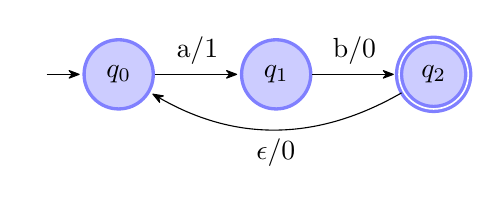
\begin{tikzpicture}[shorten >=1pt,node distance=2cm,on grid,>={Stealth[round]},
      every state/.style={draw=blue!50,very thick,fill=blue!20}, initial text=]

      \node[state,initial]            (q_0)                      {$q_0$};
      \node[state]                    (q_1) [right=of q_0]       {$q_1$};
      \node[state,accepting]          (q_2) [right=of q_1]       {$q_2$};

      \path[->] (q_0) edge              node      [above]           {a/1} (q_1)
      (q_1) edge              node      [above]           {b/0} (q_2)
      (q_2) edge [bend left]  node      [below]           {$\epsilon$/0} (q_0);
    \end{tikzpicture}
    \caption{$\aut_{ab\{1,100\}}$ where $R=(r_1)$ and $\theta = 1\leq r_1 \leq 100$}
    \label{fig:cefa1}
  \end{figure}
\end{example}
The example \ref{eg:1} gives a general picture of constructing a CEFA for a specific extended regex. Firstly, we build an NFA from the extended regex $\regex$
(e.g, To construct CEFA in example \ref{eg:1}, we firstly construct an NFA with
transition to be $q_0\xrightarrow{a} q_1\xrightarrow{b}q_2\xrightarrow{\epsilon}
  q_0$ and $I={q_0}, F={q_2}$). Secondly, we extend NFA to CEFA by adding
registers to $R$ and vectors $\bar{v}$ to each transition (e.g., we secondly add a
register $r_1$ to store repetition times and add vector $(1)$ to transition
$q_0\xrightarrow{a}q_1$ to update the repetition time). Finally, we set the
linear arithmetic $\theta$ carefully to restrict the accepted word to be
included in $\lan(\regex)$ (e.g., we finally set $\theta = 1\leq r_1\geq 100$ to
restrict the repetition times to $[1,100]$). Besides the special
operation repetition, other basic automaton operations are non-trivial. We individually discuss operations repetition, concatenation,
union, intersection, complement, and Kleene.

\subsection{Repetition}\label{subsec:rep}
Given a CEFA $\aut = (Q,\Sigma,\delta,I,F,R,\theta)$, its repetition with lower bound $l$ and upper bound $k$  is defined as $\aut_{rep} = (Q, \Sigma, \delta', I, F, R\cup\{r'\}, \theta\wedge l\leq r'\leq k )$ where
\begin{itemize}
  \item $r'$ is the new register,
  \item and $\delta'$ is composed by transitions $q\xrightarrow[(v_1, \cdots, v_n, 0)]{a} q'$ for all transitions $q\xrightarrow[(v_1, \cdots, v_n)]{a} q' \in \delta$, and transitions $q_m\xrightarrow[0_{n}\cdot 1]{\epsilon} q_0$  for all $q_m\in F$ and $q_0\in I$,
\end{itemize}
\begin{figure}[h]
  \begin{subfigure}{0.20\textwidth}
    \centering
    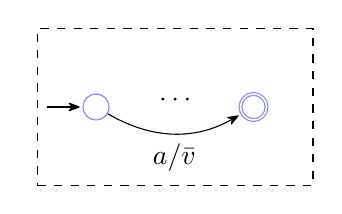
\begin{tikzpicture}[shorten >=1pt,node distance=2cm,on grid,>={Stealth[round]},
      every fit/.style={draw,minimum height=2cm,minimum width=3.5cm,dashed},
      every state/.style={draw=blue!50,minimum size = 0.1cm}, initial text=]
      \node[state, initial]   (q_0) {};
      \node[state, accepting]    (q_1) [right=of q_0] {};
      \path[->] (q_0) edge [bend right] node [below] {$a/\bar{v}$} (q_1);
      \node [fit=(q_0) (q_1)] {$\cdots$};
    \end{tikzpicture}
    \caption{The CEFA $\aut$}
  \end{subfigure}
  \begin{subfigure}{0.20\textwidth}
    \centering
    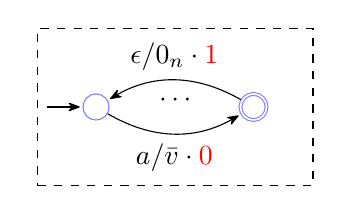
\begin{tikzpicture}[shorten >=1pt,node distance=2cm,on grid,>={Stealth[round]},
      every fit/.style={draw,minimum height=2cm,minimum width=3.5cm,dashed},
      every state/.style={draw=blue!50,minimum size = 0.1cm}, initial text=]
      \node[state, initial]   (q_0) {};
      \node[state, accepting]    (q_1) [right=of q_0] {};
      \path[->]
      (q_0) edge [bend right] node [below] {$a/\bar{v}\cdot \red{0}$} (q_1)
      (q_1) edge [bend right] node [above] {$\epsilon /0_n\cdot \red{1}$} (q_0);
      \node [fit=(q_0) (q_1)] {$\cdots$};
    \end{tikzpicture}
    \caption{The repetition of $\aut$}
  \end{subfigure}
  \caption{Repetition}
  \label{fig:rep}
\end{figure}
Figure \ref{fig:rep} illustrates the transition relation between $\aut$ and $\aut_{rep}$. Informally, $\aut_{rep}$ add a register $r_{n+1}$ to store the repetition time and update the repetition time on the transitions starting from the initial state. $\aut_{rep}$ add formula $l\leq r_{n+1}\leq k$ to ensure the repetition time is greater or equal to $l$ and less or equal to $k$.

\subsection{Concatenation}\label{subsec:con}
Given two CEFA $\aut_1 = (Q_1, \Sigma, \delta_1, I_1, F_1, R_1, \theta_1)$ and $\aut_2 = (Q_2, \Sigma, \delta_2,$ $I_2, F_2, R_2, \theta_2)$ where $R_1\cap R_2= \emptyset$ and $|R_1|=m,|R_2|=n$, the concatenation is defined as $\aut_{con}=(Q_1\cup Q_2, \Sigma, \delta', I_1, F_2, R_1\cup R_2, \theta_1\wedge\theta_2)$ where $\delta'$ is composed by
\begin{itemize}
  \item $q_1\xrightarrow[\bar{v_1}\cdot 0_n]{a} q_1'$ for each transition $q_1\xrightarrow[\bar{v_1}]{a} q_1' \in \delta_1$,
  \item $q_2\xrightarrow[0_m\cdot\bar{v_2}]{a} q_2'$ for each transition $q_2\xrightarrow[\bar{v_2}]{a} q_2' \in \delta_2$,
  \item and $q_1\xrightarrow[0_{m+n}]{\epsilon} q_2$ for each $q_1\in F_1$ and $q_2 \in I_2$.
\end{itemize}
\begin{figure}[h]
  \centering
  \begin{subfigure}{0.20\textwidth}
    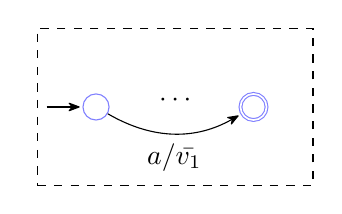
\begin{tikzpicture}[shorten >=1pt,node distance=2cm,on grid,>={Stealth[round]},
      every fit/.style={draw,minimum height=2cm,minimum width=3.5cm,dashed},
      every state/.style={draw=blue!50,minimum size = 0.1cm}, initial text=]
      \node[state, initial]   (q_0) {};
      \node[state, accepting]    (q_1) [right=of q_0] {};
      \path[->] (q_0) edge [bend right] node [below] {$a/\bar{v_1}$} (q_1);
      \node [fit=(q_0) (q_1)] {$\cdots$};
    \end{tikzpicture}
    \caption{The CEFA $\aut_1$}
  \end{subfigure}
  \begin{subfigure}{0.20\textwidth}
    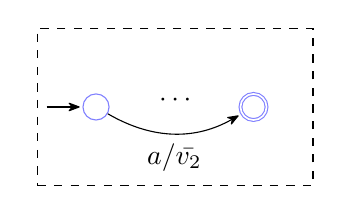
\begin{tikzpicture}[shorten >=1pt,node distance=2cm,on grid,>={Stealth[round]},
      every fit/.style={draw,minimum height=2cm,minimum width=3.5cm,dashed},
      every state/.style={draw=blue!50,minimum size = 0.1cm}, initial text=]
      \node[state, initial]   (q_0) {};
      \node[state, accepting]    (q_1) [right=of q_0] {};
      \path[->] (q_0) edge [bend right] node [below] {$a/\bar{v_2}$} (q_1);
      \node [fit=(q_0) (q_1)] {$\cdots$};
    \end{tikzpicture}
    \caption{The CEFA $\aut_2$}
  \end{subfigure}
  \begin{subfigure}{0.4\textwidth}
    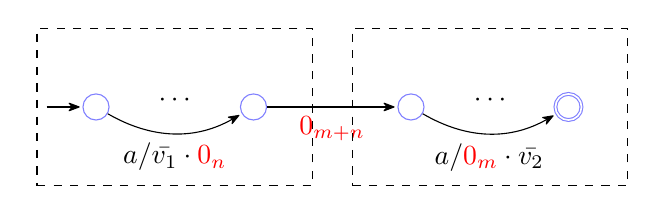
\begin{tikzpicture}[shorten >=1pt,node distance=2cm,on grid,>={Stealth[round]},
      every fit/.style={draw,minimum height=2cm,minimum width=3.5cm,dashed},
      every state/.style={draw=blue!50,minimum size = 0.1cm}, initial text=]
      \node[state, initial]   (q_0) {};
      \node[state]    (q_1) [right=of q_0] {};
      \node[state]    (q_2) [right=of q_1] {};
      \node[state, accepting]    (q_3) [right=of q_2] {};
      \path[->]
      (q_0) edge [bend right] node [below] {$a/\bar{v_1}\cdot \red{0_n}$} (q_1)
      (q_1) edge node [below] {$\red{0_{m+n}}$} (q_2)
      (q_2) edge [bend right] node [below] {$a/\red{0_m}\cdot \bar{v_2}$} (q_3);
      \node [fit=(q_0) (q_1)] {$\cdots$};
      \node [fit=(q_2) (q_3)] {$\cdots$};
    \end{tikzpicture}
    \caption{The concatenation of $\aut_1$ and $\aut_2$}
  \end{subfigure}
  \caption{Concatenation}
  \label{fig:con}
\end{figure}
Figure \ref{fig:con} outlines the vector change on transitions when concatenating two CEFA. Without losing information, $\aut_{con}$ contains all registers in $\aut_1$ and $\aut_2$. Furthermore, $\aut_{con}$ update registers' value of $\aut_1$ and $\aut_2$ separately: $\aut_{con}$ only update registers of $R_1$ on the transitions of $\aut_1$ and update registers of $R_2$ on the transition of $\aut_2$. $\theta'$ is the conjunction of $\theta_1$ and $\theta_2$ to make sure all linear constraints in $\aut_1$ and $\aut_2$ are satisfiable.
\subsection{Intersection}\label{subsec:inter}
Given two CEFA $\aut_1 = (Q_1, \Sigma, \delta_1, I_1, F_1, R_1, \theta_1)$ and $\aut_2 = (Q_2, \Sigma, \delta_2,$ $I_2, F_2, R_2, \theta_2)$ with $R_1\cap R_2 = \emptyset$, the intersection is defined as $\aut_{inter} = (Q_1\times Q_2, \Sigma, \delta', I_1\times I_2, F_1\times F_2, R_1\cup R_2, \theta_1\wedge \theta_2)$ where $\delta'$ is composed by
\begin{itemize}
  \item transitions $(q_1,q_2)\xrightarrow[\bar{v_1}\cdot\bar{v_2}]{a} (q_1',q_2')$ when both transition $q_1\xrightarrow[\bar{v_1}]{a}q_1'$ and transition $q_2\xrightarrow[\bar{v_2}]{a}q_2'$ exist in $\delta$.
\end{itemize}
\begin{figure}[h]
  \centering
  \begin{subfigure}{0.20\textwidth}
    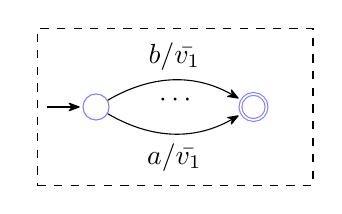
\begin{tikzpicture}[shorten >=1pt,node distance=2cm,on grid,>={Stealth[round]},
      every fit/.style={draw,minimum height=2cm,minimum width=3.5cm,dashed},
      every state/.style={draw=blue!50,minimum size = 0.1cm}, initial text=]
      \node[state, initial]   (q_0) {};
      \node[state, accepting]    (q_1) [right=of q_0] {};
      \path[->]
      (q_0) edge [bend right] node [below] {$a$/$\bar{v_1}$} (q_1)
      (q_0) edge [bend left] node [above] {$b$/$\bar{v_1}$} (q_1);
      \node [fit=(q_0) (q_1)] {$\cdots$};
    \end{tikzpicture}
    \caption{The CEFA $\aut_1$}
  \end{subfigure}
  \begin{subfigure}{0.20\textwidth}
    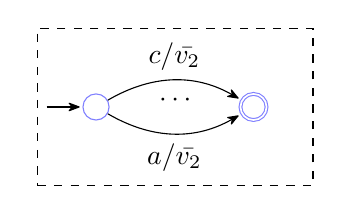
\begin{tikzpicture}[shorten >=1pt,node distance=2cm,on grid,>={Stealth[round]},
      every fit/.style={draw,minimum height=2cm,minimum width=3.5cm,dashed},
      every state/.style={draw=blue!50,minimum size = 0.1cm}, initial text=]
      \node[state, initial]   (q_0) {};
      \node[state, accepting]    (q_1) [right=of q_0] {};
      \path[->]
      (q_0) edge [bend right] node [below] {$a$/$\bar{v_2}$} (q_1)
      (q_0) edge [bend left] node [above] {$c$/$\bar{v_2}$} (q_1);
      \node [fit=(q_0) (q_1)] {$\cdots$};
    \end{tikzpicture}
    \caption{The CEFA $\aut_2$}
  \end{subfigure}
  \begin{subfigure}{0.4\textwidth}
    \centering
    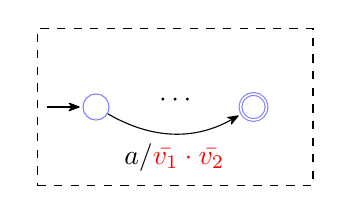
\begin{tikzpicture}[shorten >=1pt,node distance=2cm,on grid,>={Stealth[round]},
      every fit/.style={draw,minimum height=2cm,minimum width=3.5cm,dashed},
      every state/.style={draw=blue!50,minimum size = 0.1cm}, initial text=]
      \node[state, initial]   (q_0) {};
      \node[state, accepting]    (q_3) [right=of q_0] {};
      \path[->]
      (q_0) edge [bend right] node [below] {$a$/\red{$\bar{v_1}\cdot \bar{v_2}$}} (q_3);
      \node [fit=(q_0) (q_3)] {$\cdots$};
    \end{tikzpicture}
    \caption{The intersection of $\aut_1$ and $\aut_2$}
  \end{subfigure}
  \caption{Intersection}
  \label{fig:inter}
\end{figure}
The transition relation of $\aut_1,\aut_2$ and their intersection is displayed by Figure \ref{fig:inter}. The intersection of CEFA is similar to the intersection of NFA, except that the intersection of CEFA intersects registers updates and linear arithmetic.
\subsection{Union}\label{subsec:union}
Given two CEFA $\aut_1 = (Q_1, \Sigma, \delta_1, I_1, F_1, R_1, \theta_1)$ and $\aut_2 = (Q_2, \Sigma, \delta_2,$ $I_2, F_2, R_2, \theta_2)$ with $R_1\cap R_2 = \emptyset$ and $|R_1|=m,|R_2|=n$, the union is defined as $\aut_{union} = (Q_1\cup Q_2, \Sigma, \delta', \{q_0\}, F_1\cup F_2, R_1\cup R_2\cup (r', r''), \theta')$ where $\delta'$ is composed by
\begin{itemize}
  \item transitions $q_0\xrightarrow[0_{m+n}\cdot(1,0)]{\epsilon}q_1$ for all $q_1\in I_1$,
  \item transitions $q_0\xrightarrow[0_{m+n}\cdot(0,1)]{\epsilon}q_2$ for all $q_2\in I_2$,
  \item transitions $q_1\xrightarrow[\bar{v_1}0_{n+2}]{a} q_1'$ for all $q_1\xrightarrow[\bar{v_1}]{a} q_1'\in \delta_1$,
  \item transitions $q_2\xrightarrow[0_m\bar{v_2}0_2]{a} q_2'$ for all $q_2\xrightarrow[\bar{v_2}]{a} q_2'\in \delta_2$,
\end{itemize}
and 
\begin{itemize}
  \item $r'$ and $r''$ are new registers,
  \item $q_0$ is a new state where $q_0\not\in Q_1$ and $q_0\not\in Q_2$,
  \item $\theta_{tmp} = (r'>0\wedge\theta_1)\vee(r''>0\wedge\theta_2)$, $\theta'$ is constructed differently in four cases:
  \begin{itemize}
    \item [-]$I_1\cap F_1=\emptyset$ and $I_2\cap F_2=\emptyset$: $\theta'$ = $\theta_{tmp}$;
    \item [-]$I_1\cap F_1\not=\emptyset$ and $I_2\cap F_2=\emptyset$: $\theta'$ = $\theta_{tmp}\vee (r'==0\wedge r''==0\wedge\theta_1)$;
    \item [-]$I_1\cap F_1=\emptyset$ and $I_2\cap F_2\not=\emptyset$: $\theta'$ = $\theta_{tmp}\vee (r'==0\wedge r''==0\wedge\theta_2)$;
    \item [-]$I_1\cap F_1\not=\emptyset$ and $I_2\cap F_2\not=\emptyset$: $\theta'$ = $\theta_{tmp}\vee (r'==0\wedge r''==0\wedge(\theta_1\vee\theta_2))$;
  \end{itemize}
\end{itemize}
\begin{figure}[h]
  \centering
  \begin{subfigure}{0.20\textwidth}
    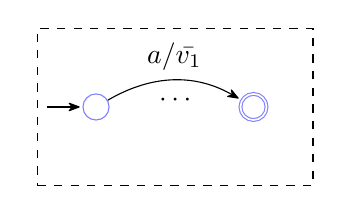
\begin{tikzpicture}[shorten >=1pt,node distance=2cm,on grid,>={Stealth[round]},
      every fit/.style={draw,minimum height=2cm,minimum width=3.5cm,dashed},
      every state/.style={draw=blue!50,minimum size = 0.1cm}, initial text=]
      \node[state, initial]   (q_0) {};
      \node[state, accepting]    (q_1) [right=of q_0] {};
      \path[->]
      (q_0) edge [bend left] node [above] {$a$/$\bar{v_1}$} (q_1);
      \node [fit=(q_0) (q_1)] {$\cdots$};
    \end{tikzpicture}
    \caption{The CEFA $\aut_1$}
  \end{subfigure}
  \begin{subfigure}{0.20\textwidth}
    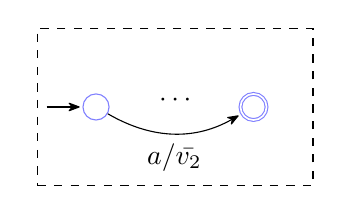
\begin{tikzpicture}[shorten >=1pt,node distance=2cm,on grid,>={Stealth[round]},
      every fit/.style={draw,minimum height=2cm,minimum width=3.5cm,dashed},
      every state/.style={draw=blue!50,minimum size = 0.1cm}, initial text=]
      \node[state, initial]   (q_0) {};
      \node[state, accepting]    (q_1) [right=of q_0] {};
      \path[->]
      (q_0) edge [bend right] node [below] {$a$/$\bar{v_2}$} (q_1);
      \node [fit=(q_0) (q_1)] {$\cdots$};
    \end{tikzpicture}
    \caption{The CEFA $\aut_2$}
  \end{subfigure}
  \begin{subfigure}{0.4\textwidth}
    \centering
    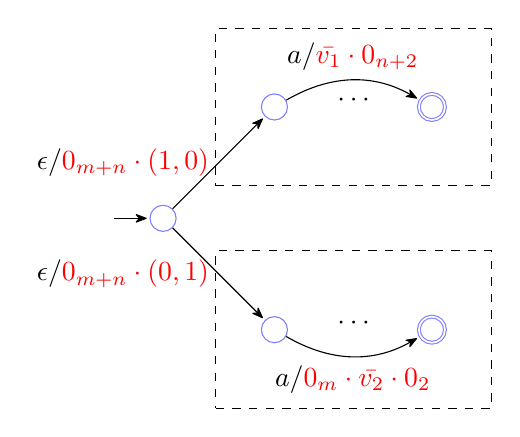
\begin{tikzpicture}[shorten >=1pt,node distance=2cm,on grid,>={Stealth[round]},
      every fit/.style={draw,minimum height=2cm,minimum width=3.5cm,dashed},
      every state/.style={draw=blue!50,minimum size = 0.1cm}, initial text=]
      \node[state, initial]   (q_0) {};
      \node[state]   (q_1) [above right=of q_0] {};
      \node[state, accepting]   (q_1') [right=of q_1] {};
      \node[state]   (q_2) [below right=of q_0] {};
      \node[state, accepting]   (q_2') [right=of q_2] {};
      \path[->]
      (q_0) edge node [left] {$\epsilon/\red{0_{m+n}\cdot(1,0)}$} (q_1)
      (q_0) edge node [left] {$\epsilon/\red{0_{m+n}\cdot(0,1)}$} (q_2)
      (q_1) edge [bend left] node [above] {$a$/\red{$\bar{v_1}\cdot 0_{n+2}$}} (q_1')
      (q_2) edge [bend right] node [below] {$a$/\red{$0_m\cdot \bar{v_2}\cdot 0_2$}} (q_2');
      \node [fit=(q_1) (q_1')] {$\cdots$};
      \node [fit=(q_2) (q_2')] {$\cdots$};
    \end{tikzpicture}
    \caption{The union of $\aut_1$ and $\aut_2$}
  \end{subfigure}
  \caption{Union}
  \label{fig:union}

\end{figure}
The Union of two CEFA is shown in Figure \ref{fig:union}. To simulate the semantics of the union, we add an initial state $q_0$ and transitions from $q_0$ to initial states of $\aut_1$ and $\aut_2$ to randomly choose one automaton. The values of $r'$ and $r''$ distinguish which automaton we run. In the construction above, $r'>0$ means that we choose $\aut_1$ to run a word, $r''>0$ implies that we select $r''$ to run a word, and $r'==0\wedge r''=0$ means that we decide to run word $\epsilon$.

\subsection{Complement}\label{subsec:comp}
We use the function $nfa$ to return the NFA form of a CEFA. More precisely, given a CEFA $\aut = (Q, \Sigma, I, F, \delta, R, \theta)$, $nfa(\aut)$ is an NFA tuple $(Q, \Sigma, \delta', I, F)$  where $\delta'$ comprises transition $(q, a, q')$ for $(q, a, q', \bar{v})\in \delta$ . Similarly, the function $cefa(\aut)$ is used to return the CEFA form of an NFA: $cefa(\aut_{nfa}) = (Q, \Sigma, I, F, \delta, \emptyset, true)$ for $\aut_{nfa} = (Q, \Sigma, I, F, \delta')$ where $\delta$ comprises transition $(q, a, q', \emptyset)$ for $(q, a, q')\in \delta'$. \verb|uion| denotes the CEFA operation union.

Given a CEFA $\aut = (Q,\Sigma, \delta, I, F, R, \theta)$, the complement of $\aut$ is defined as $\aut_{comp} = \verb|union|(\aut_{NFA}^C, \aut_{negf})$ where $\aut_{negf} = \\(Q,\Sigma, \delta, I, F, R, \neg\theta)$ and $\aut_{NFA}^C$ is obtained by three steps:
\begin{itemize}
  \item compute the NFA form $\aut_n = nfa(\aut) = (Q,\sigma, \delta', I, F)$,
  \item the complement of $\aut_n$ is $\aut_n^C = (Q, \sigma, \delta', F, I)$,
  \item extend $\aut_n^C$ to CEFA form $\aut_{NFA}^C = cefa(\aut_n^C)$.
\end{itemize}
\begin{figure}[h]
  \begin{subfigure}{0.40\textwidth}
    \centering
    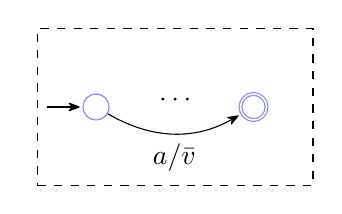
\begin{tikzpicture}[shorten >=1pt,node distance=2cm,on grid,>={Stealth[round]},
      every fit/.style={draw,minimum height=2cm,minimum width=3.5cm,dashed},
      every state/.style={draw=blue!50,minimum size = 0.1cm}, initial text=]
      \node[state, initial]   (q_0) {};
      \node[state, accepting]    (q_1) [right=of q_0] {};
      \path[->] (q_0) edge [bend right] node [below] {$a/\bar{v}$} (q_1);
      \node [fit=(q_0) (q_1)] {$\cdots$};
    \end{tikzpicture}
    \caption{The CEFA $\aut$}
  \end{subfigure}
  \begin{subfigure}{0.20\textwidth}
    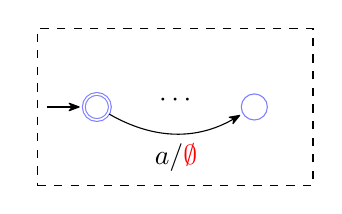
\begin{tikzpicture}[shorten >=1pt,node distance=2cm,on grid,>={Stealth[round]},
      every fit/.style={draw,minimum height=2cm,minimum width=3.5cm,dashed},
      every state/.style={draw=blue!50,minimum size = 0.1cm}, initial text=
      ]
      \node[state, initial, accepting]   (q_0) {};
      \node[state]    (q_1) [right=of q_0] {};
      \path[->]
      (q_0) edge [bend right] node [below] {$a$/\red{$\emptyset$}} (q_1);
      \node [fit=(q_0) (q_1)] {$\cdots$};
    \end{tikzpicture}
    \caption{The CEFA $\aut_{NFA}^C$}
  \end{subfigure}
  \begin{subfigure}{0.20\textwidth}
    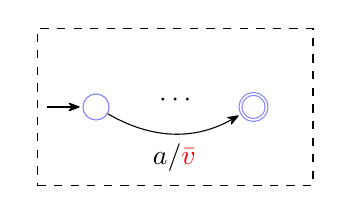
\begin{tikzpicture}[shorten >=1pt,node distance=2cm,on grid,>={Stealth[round]},
      every fit/.style={draw,minimum height=2cm,minimum width=3.5cm,dashed},
      every state/.style={draw=blue!50,minimum size = 0.1cm}, initial text=]
      \node[state, initial]   (q_0) {};
      \node[state, accepting]    (q_1) [right=of q_0] {};
      \path[->]
      (q_0) edge [bend right] node [below] {$a$/\red{$\bar{v}$}} (q_1);
      \node [fit=(q_0) (q_1)] {$\cdots$};
    \end{tikzpicture}
    \caption{The CEFA $\aut_{negf}$}
  \end{subfigure}
  \caption{Complement}
  \label{fig:comp}
\end{figure}
As Figure \ref{fig:comp} shows, the complement of CEFA is the union of $\aut_{NFA}^C$ and $\aut_{negf}$. $\aut_{NFA}^C$ accepts words that $nfa(\aut)$ does not accept and $\aut_{negf}$ accepted words might be accepted by the $nfa(\aut)$ but not satisfy linear constraints $\theta$.
\subsection{Kleene}\label{subsec:klee}
The construction of Kleene is trivial. Given a CEFA $\aut = (Q,\Sigma,\delta,I,F,R,\theta)$ with $|R|=n$, the Kleene of $\aut_{Kleene}$ is defined as $(Q,\Sigma,\delta',I,F,R,\theta)$ where $\delta'$ comprises all transitions in $\delta$ and new transitions $q_f\xrightarrow[0_n]{\epsilon} q_0$ for each $q_0\in I$ and $q_f\in F$.

\subsection{From Extended Regex to CEFA} \label{subsec:regex2cefa}
\highlight{Basis}: The basis has three parts with empty registers and valid linear arithmetic, shown in Fig. \ref{fig:basis}. In part \ref{fig:basis:a}, we see how to handle the expression $\epsilon$. The language of the automaton is easily seen to be $\{\epsilon\}$ since the only path from the start state to an accepting state
is labeled $\epsilon$. Part \ref{fig:basis:b} gives the CEFA for a regular expression $\mathbf{a}$. The language of this CEFA consists of the single string $a$, which is also $\lan(\mathbf{a})$. Finally, part \ref{fig:basis:c} shows the construction for $\emptyset$. There are no paths from the initial state to the accepting state.
\begin{figure}[h]
  \centering
  \begin{subfigure}{0.13\textwidth}
    \centering
    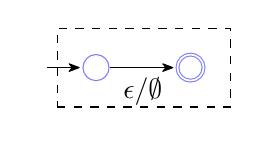
\begin{tikzpicture}[shorten >=1pt,node distance=1.2cm,on grid,>={Stealth[round]},
      every fit/.style={draw,minimum height=1.0cm,minimum width=2.2cm,dashed},
      every state/.style={draw=blue!50,minimum size = 0.1cm}, initial text=]
      \node[state, initial]   (q_0) {};
      \node[state, accepting]    (q_1) [right=of q_0] {};
      \path[->] (q_0) edge node [below] {$\epsilon/\emptyset$} (q_1);
      \node [fit=(q_0) (q_1)] {};
    \end{tikzpicture}
    \caption{}
    \label{fig:basis:a}
  \end{subfigure}
  \begin{subfigure}{0.13\textwidth}
    \centering
    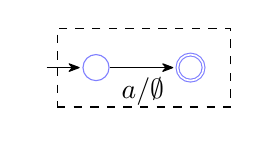
\begin{tikzpicture}[shorten >=1pt,node distance=1.2cm,on grid,>={Stealth[round]},
      every fit/.style={draw,minimum height=1.0cm,minimum width=2.2cm,dashed},
      every state/.style={draw=blue!50,minimum size = 0.1cm}, initial text=]
      \node[state, initial]   (q_0) {};
      \node[state, accepting]    (q_1) [right=of q_0] {};
      \path[->] (q_0) edge node [below] {$a/\emptyset$} (q_1);
      \node [fit=(q_0) (q_1)] {};
    \end{tikzpicture}
    \caption{}
    \label{fig:basis:b}
  \end{subfigure}
  \begin{subfigure}{0.13 \textwidth}
    \centering
    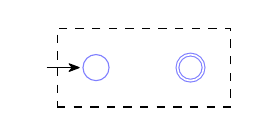
\begin{tikzpicture}[shorten >=1pt,node distance=1.2cm,on grid,>={Stealth[round]},
      every fit/.style={draw,minimum height=1.0cm,minimum width=2.2cm,dashed},
      every state/.style={draw=blue!50,minimum size = 0.1cm}, initial text=]
      \node[state, initial]   (q_0) {};
      \node[state, accepting]    (q_1) [right=of q_0] {};
      \node [fit=(q_0) (q_1)] {};
    \end{tikzpicture}
    \caption{}
    \label{fig:basis:c}
  \end{subfigure}
  \caption{The basis of the construction of a CEFA from extended regex}
  \label{fig:basis}
\end{figure}\\
\highlight{Induction}: Given the CEFA of the subexpression, we construct the CEFA in five cases:
\begin{enumerate}
  \item The expression is $\regex\{m,n\}$ for some smaller expression $\regex$. We can repeat the CEFA of $\regex$ with lower bound $m$ and upper bound $n$ as shown in section \ref{subsec:rep}.
  \item The expression is $\regex_1\cdot\regex_2$ for some smaller expression $\regex_1$ and $\regex_2$. We can concatenate the CEFA of $\regex_1$ and the CEFA of $\regex_2$ as shown in section \ref{subsec:con}.
  \item The expression is $\regex_1\times \regex_2$ for some smaller expression $\regex_1$ and $\regex_2$. We can intersect the CEFA of $\regex_1$ and the CEFA of $\regex_2$ as shown in section \ref{subsec:inter}.
  \item The expression is $\regex_1 + \regex_2$ for some smaller expression $\regex_1$ and $\regex_2$. We can union the CEFA of $\regex_1$ and the CEFA of $\regex_2$ as shown in section \ref{subsec:union}.
  \item The expression is $\regex*$ for some smaller expression $\regex$. We can construct the Kleene Star of the CEFA of $\regex$  as shown in section \ref{subsec:klee}.
  \item The expression is $\regex^C$ for some smaller expression $\regex$. We can construct the complement of the CEFA of $\regex$  as shown in section \ref{subsec:comp}
\end{enumerate}
\highlight{Special Case}: When the expression $\regex$ contains nested repetition, we firstly write $\regex$ to a new regex $\regex'$ without nested repetition. Then we build the CEFA of the new expression $\regex'$ by basis and induction steps.

\section{Solve String Constraints with Large Repetition Bound} \label{sec:solve}
Following the decision procedure defined in the paper \cite{atva2020}, we propose an efficient algorithm to solve string constraints by CEFA. Firstly, we replace all length operations $i=\strlen{x}$ to pre-images, and intersect these pre-images to $lenAut_x$. Then for each term $x$, we genearte CEFAs from all regular expressiones $\regex$ in all terms $x\in \regex$, and intersect the CEFAs with $lenAut_x$ to get the final CEFAs. Finally, we check whether the final CEFAs is empty under the linear integer arithmetic $P$. If one of the final CEFAs is empty, the string constraints are unsatisfiable. Otherwise, the string constraints are satisfiable. The high-level algorithm is shown in the Algorithm \ref{alg:high}.\newline
The emptiness checking problem of CEFAs under linear integer arithmetic $P$ is theoretically pspace-complete\cite{atva2020}. To solve it efficiently for practical example, we add some heuristics. The details of the heuristics are shown in Algorithm \ref{alg:emptiness}.
% \pagebreak
\subsection{High-level algorithm}
\begin{algorithm}
  \caption{High-level algorithm}
  \label{alg:high}
  \begin{algorithmic}[1]
    \Require  Conjunction $\varphi$ of the form $x\in \regex$, and conjunction of linear integer arithmetic $P$ over string lengths
    \Ensure \emph{sat} or \emph{unsat}
    \Statex
    \ForAll{length operation $i = \strlen{x}$} \label{alg:high:line1}
      \State $lenAut_{x} \leftarrow \aut_{allstring}$ \label{alg:high:line2}
      \State Let $\aut_{i}$ be the pre-image of length operation with length $i$ \label{alg:high:line3}
      \State $lenAut_{x} \leftarrow lenAut_{x} \times \aut_{i}$ \label{alg:high:line4}
    \EndFor \label{alg:high:line5}
    \State $atomAuts \leftarrow \emptyset$ \label{alg:high:line6}
    \ForAll{string variables $x$ occurring in $\varphi$} 
    \State Let $S$ be the set of all regexes $\regex$ in all terms $x \in \regex$ 
    \State CEFA $\aut_x \leftarrow$ intersection of $lenAut_x$ and all CEFAs corresponding to regexes in $S$
    \If{$nfa(\aut_x)$ is empty} \label{alg:high:line5}
      \State \textbf{return} \emph{unsat}
    \EndIf
    \State $atomAuts \leftarrow atomAuts \cup \{\aut_x\}$ 
    \EndFor
    \If{$\algfun{isEmpty}(atomAuts, P)$ }
      \State \textbf{return} \emph{unsat}
    \Else 
      \State \textbf{return} \emph{sat}
    \EndIf
  \end{algorithmic}
\end{algorithm}
The pseudocode presented in Algorithm \ref{alg:high} outlines the framework of our solving process. The implemented details are eliminated for clarity. From line \ref{alg:high:line1} to line \ref{alg:high:line5}, we construct the CEFAs of all length operations $i = \strlen{x}$ occurring in $\varphi$. The CEFA $lenAut_x$ is the automaton reserving all length information on $x$. $lenAut_x$ is initiated to accept all strings at line \ref{alg:high:line2}. And for each length operation $i = \strlen{x}$, we construct the pre-image of the length operation at line \ref{alg:high:line3}. Then we intersect $lenAut_x$ with the pre-image at line \ref{alg:high:line4}. Note that the final $lenAut_x$ is the intersection of many pre-images.\newline
In the following steps, we call a CEFA to be \emph{atomic} if we will not operate it anymore. The set $atomAuts$ is the set of all atomic CEFAs for all terms $x$ occurring in $\varphi$, and it is initiated to empty set at line \ref{alg:high:line6}. From line \ref{alg:high:line6} to line 14, we construct the atomic CEFAs of all string variables $x$ occurring in $\varphi$. For each string variable $x$, we construct the CEFA $\aut_x$ by intersecting $lenAut_x$ and all CEFAs corresponding to regexes in $S$. If the NFA form of $\aut_x$ is empty (i.e., the NFA accepts no word), we return $unsat$ directly because the NFA form is an over-approximation of CEFA. Otherwise, we add $\aut_x$ to $atomAuts$ at line 9.\newline
After obtaining the atomic CEFAs of all string terms, we check whether the atomic CEFAs are empty under the linear integer arithmetic $P$ at line 15. If the atomic CEFAs are empty, we return $unsat$. Otherwise, we return $sat$. The emptiness checking is complex, and we will discuss its details in the following subsection.\newline


\subsection{Emptyness Checking}
As mentioned, the emptiness checking problem of CEFA under linear integer arithmetic $P$ is theoretically pspace-complete \cite{atva2020}. In our previous research, we rewrote CEFA to an infinite system and used a model-checking tool \emph{NuSMV} to solve it. In this paper, we use a more efficient method to solve the emptiness checking problem. The details are shown in Algorithm \ref{alg:emptiness}.\newline
The input CEFAs may have many transitions and registers, so the emptiness checking problem is hard to solve. We simplify the CEFAs at line 1. The simplification is to remove all duplicated transitions and registers in the CEFAs. The simplification is implemented by Algorithm \ref{alg:simplify}. Then we try to find a solution by under-approximation at line 3. The under-approximation is implemented by Algorithm \ref{alg:underApprox}. If we find a solution, the CEFAs under linear integer arithmetic $P$ are not empty. So we return $false$ at line 5. We will try many times until we find a solution or reach $MaxBound$. Otherwise, we try to find an unsat core by over-approximation at line 8. The over-approximation is implemented by Algorithm \ref{alg:overApprox}. If we discover an unsat core, we know that the CEFAs under $P$ are empty, and we return $true$ at line 10. Suppose both under- and over-approximation do not make sense. In that case, we compute the Parikh images\cite{parikh_2005} of the simplified CEFAs and check if the Parikh images in conjunction with $P$ are satisfiable at line 12. The unsatisfiability implies emptiness directly.
\begin{algorithm}
  \caption{ $\algfun{isEmpty}(auts, P)$}
  \label{alg:emptiness}
  \begin{algorithmic}[1]
    \Require CEFAs $auts$ and linear integer arithmetic $P$
    \Ensure $true$ or $false$
    \Statex
    \State $simpliAuts \leftarrow \algfun{simplify}(auts)$
    \For{$bound \gets 1, MaxBound$ }
      \State $\varphi_{under}\gets \algfun{underApprox}(simpliAuts, bound)$
      \If{$\varphi_{under}\wedge P$ is sat}
        \State \textbf{return} $false$
      \EndIf
    \EndFor
    \State $\varphi_{over}\gets \algfun{overApprox}(simpliAuts)$
    \If{$\varphi_{over}\wedge P$ is unsat}
      \State \textbf{return} $true$
    \EndIf
    \State $\varphi \gets \algfun{parikhImage}(simpliAuts)$
    \If{$\varphi\wedge P$ is unsat}
      \State \textbf{return} $true$
    \Else
      \State \textbf{return} $false$
    \EndIf
  \end{algorithmic}
\end{algorithm}
\subsection{Simplification of CEFA}
The main idea of simplification is to remove duplicated transitions and registers. In emptiness checking Algorithm \ref{alg:emptiness}, the vectors on the transitions are meaningful, but the letters on the transitions are not. So we see the alphabet of the CEFA as unary (i.e., the alphabet is $\{a\}$). Compared with NFA, the vectors in the CEFA are the letters in the NFA, and the vector $\myvec{0}_n$ is seen as $\epsilon$. Based on the similarity between NFA and CEFA, firstly, determinization and minimization \cite{aut_hopcraft} are applied to simplify the CEFA. Then we merge the registers having the same updating at all transitions and get the final CEFA. The main simplification framework is shown in Algorithm \ref{alg:simplify}, and some details are eliminated for simplicity.
\begin{algorithm}
  \caption{$\algfun{simplify}(auts)$}
  \label{alg:simplify}
  \begin{algorithmic}[1]
    \Require CEFAs $auts$
    \Ensure Simplified CEFAs $simpliAuts$
    \Statex
    \State $simpliAuts \gets \emptyset$
    \For{$aut \in auts$}
      \State $aut \gets \algfun{determinizeByVec}(aut)$
      \State $aut \gets \algfun{minimizeByVec}(aut)$
      \State $aut \gets \algfun{mergeRegisters}(aut)$
      \State $simpliAuts \gets simpliAuts \cup \{aut\}$
    \EndFor
    \State \textbf{return} $simpliAuts$
  \end{algorithmic}
\end{algorithm}

\subsection{Under-Approximation}
To solve the emptiness checking problem, we translate the CEFAs to linear integer arithmetic and check if the linear integer arithmetic in conjunction with $P$ is satisfiable. The main idea of under-approximation is to translate the CEFAs step by step. A string length bound controls the translation, and linear integer arithmetic is generated from low to high length bound. This section only discusses the situation where the bound is fixed. The details are shown in the Algorithm \ref{alg:underApprox}. Firstly, the linear integer arithmetic $\varphi_{under}$ is assigned to be false at line 1. Then for each CEFA, we enumerate all the accepted paths with lengths less than the bound and translate the paths to linear integer arithmetic. The linear integer arithmetic is in conjunction with $\varphi_{under}$ at line 4.
\begin{algorithm}
  \caption{$\algfun{underApprox}(auts, bound)$}
  \label{alg:underApprox}
  \begin{algorithmic}[1]
    \Require CEFAs $auts$ and length bound $bound$
    \Ensure Linear integer arithmetic $\varphi_{under}$
    \Statex
    \State $\varphi_{under} \gets false$
    \For{$aut \in auts$}
      \State Let $\varphi_{aut}$ to be the linear integer arithmetic generated by  enumerating all the paths with length less than $bound$ in $aut$
      \State $\varphi_{under} \gets \varphi_{under} \wedge \varphi_{aut}$
    \EndFor
    \State \textbf{return} $\varphi_{under}$
  \end{algorithmic}
\end{algorithm}
\subsection{Over-Approximation}
Sometimes when the bound reaches the maximum, the linear integer arithmetic $\varphi_{under}$ is still unsatisfiable. We must use over-approximation to solve the emptiness checking problem in this case. The main idea of over-approximation is to split each CEFA into sub-CEFAs, translate each sub-CEFA respectively, and finally in conjunction with the LIA of all sub-CEFAs. The details are shown in the Algorithm \ref{alg:overApprox}. Firstly, each CEFA is split into $n$ sub-CEFAs, where $n$ is the number of registers in the CEFA. The sub-CEFA has only one register. After simplifying each sub-CEFA by Algorithm \ref{alg:simplify}, the vector of each transition must be $\myvec{1}$. So the register value of each sub-CEFA equals the length of the accepted path. We apply the efficient construction of semilinear representations\cite{unary_nfa_2010} to get the linear integer arithmetic $\varphi_{over}$.
\begin{algorithm}
  \caption{$\algfun{overApprox}(auts)$}
  \label{alg:overApprox}
  \begin{algorithmic}[1]
    \Require CEFAs $auts$
    \Ensure Linear integer arithmetic $\varphi_{over}$
    \Statex
    \State $\varphi_{over} \gets true$
    \For{$aut \in auts$}
      \State Let $subAut$ be the sub-CEFA of $aut$ with only one register
      \State Let $subAut \gets \algfun{simplify}(subAut)$
      \State Let $\varphi_{subAut}$ be the linear integer arithmetic generated by efficient construction of semilinear representations
      \State $\varphi_{over} \gets \varphi_{over} \wedge \varphi_{subAut}$
    \EndFor
    \State \textbf{return} $\varphi_{over}$
  \end{algorithmic}
\end{algorithm}
\section{Implementation and Experiment} \label{sec:imp}
% % TODO: Implementation and experiment result
TODO
% We implement Algorithm \ref{alg:high} on our string solver ostrich \cite{ostrich2023}. And compare our solver with z3 on benchmark \emph{LoopBench}. The result shows that our algorithm performs better than z3.\\
% \highlight{LoopBench}: The benchmark consists of three parts:
% \begin{enumerate}
%   \item \textbf{Z3strRE}: We extract instances with repetition operator from (paper z3str3Re). z3strRE support string operation \verb|num2str| which is not supported by ostrich. So we remove these instances with \verb|num2str|.
%   \item \textbf{StackOverflow}: We extract real-world regexes from StackOverflow\cite{stackoverflow} using the tool zaligvinder\cite{zaligvinder_2021} and translate these regexes to smtlib2 format. For each regex, we generate an instance with one regular membership and a length operation.
%   \item \textbf{RegexLib}: We also extract real-world regexes from regexlib\cite{regexlib} using zaligvinder and generate instances in the same way as StackOverflow.
% \end{enumerate}
% The experimental result is shown in Table \ref{tab:res}. ostrich performs very closely on satisfiable instances and outperforms z3 on unsatisfiable instances. Furthermore, ostrich use a little more time to find the result rather than z3.
% \begin{table}[h]
%   \begin{tabular}{|l|l|l|l|l|l|}
%     \hline
%             & sat  & unsat & error & sat time & unsat time \\ \hline
%     z3      & 6995 & 5491  & 382   & 1.09s    & 0.42s      \\ \hline
%     ostrich & 6966 & 5751  & 150   & 2.82s    & 1.81s      \\ \hline
%   \end{tabular}
%   \caption{Detailed results for the LoopBench benchmark. Ostrich can solve more instances.}
%   \label{tab:res}
% \end{table}

\section{Conclusion and Future Work} \label{sec:conclu}
In this paper, we aim to solve the string constraints with large repetition time efficiently. A new automaton model CEFA is proposed to reduce the search space. Many basic operations on CEFA are non-trivial and we should formal them carefully. Moreover, we extend the algorithm in the paper \cite{atva2020} with heuristics such as under- and over-approximation. The implementation of the algorithm is done on string solver ostrich. The extensive empirical comparison against z3 over a large and diverse benchmark shows the power of our model and algorithm. In the future, we plan to explore the way to solve nested repetition and use CEFA to solve more string operations.

%%
%% The next two lines define the bibliography style to be used, and
%% the bibliography file.
\bibliographystyle{ACM-Reference-Format}
\bibliography{ref}

\end{document}

%%
%% End of file `sample-sigconf.tex'.
